% Attack chain, CVE-2026-53988: unsigned webhook -> host root.
\documentclass[border=6pt,tikz]{standalone}
\usetikzlibrary{arrows.meta,backgrounds,calc}
\definecolor{chainbg}{RGB}{250,251,253}
\definecolor{chainline}{RGB}{105,115,132}
\definecolor{atkline}{RGB}{170,60,60}
\definecolor{breakfill}{RGB}{253,232,232}
\definecolor{breakline}{RGB}{170,60,60}
\definecolor{stepfill}{RGB}{240,244,250}
\definecolor{sinkfill}{RGB}{255,238,222}
\definecolor{sinkline}{RGB}{190,115,40}
\definecolor{fixfill}{RGB}{230,246,230}
\definecolor{fixline}{RGB}{62,124,62}
\begin{document}
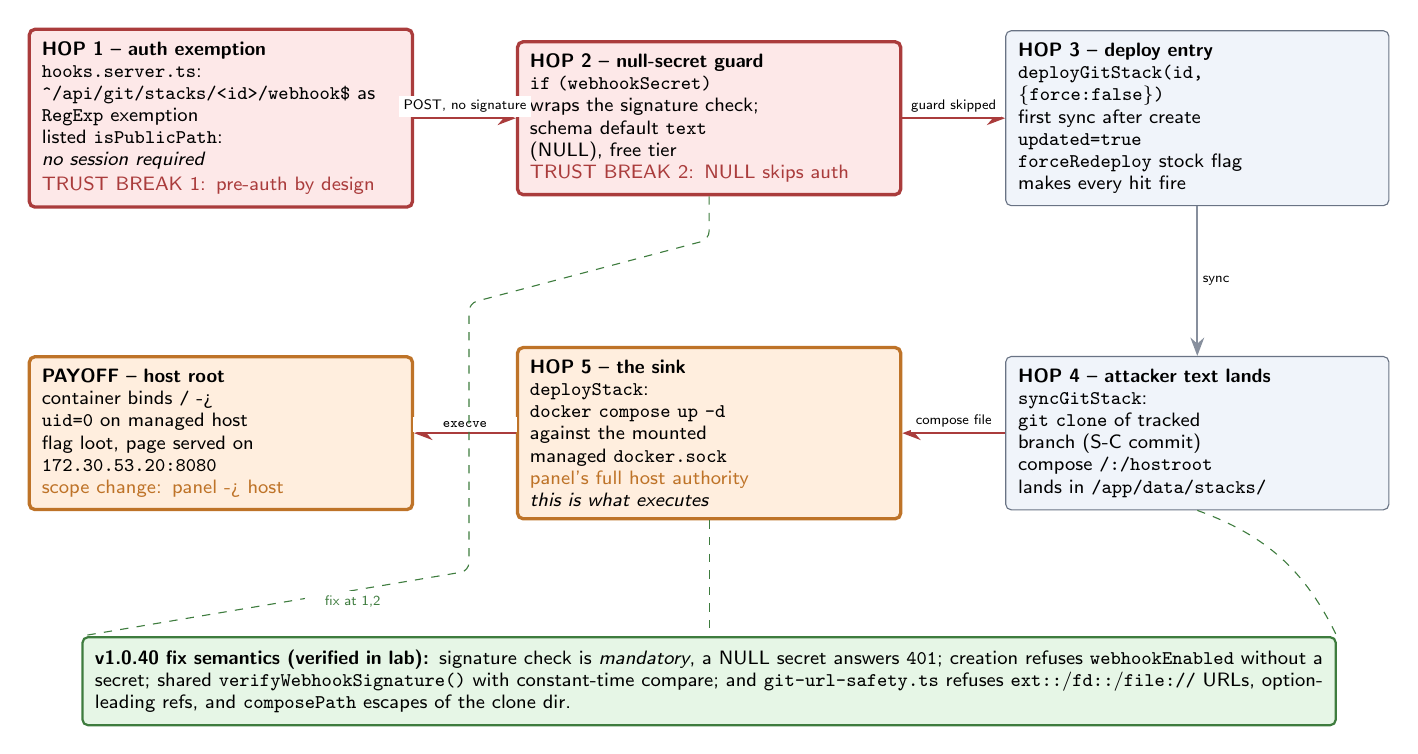
\begin{tikzpicture}[
  >=Stealth,
  box/.style={draw=chainline, fill=white, rounded corners=2pt, align=left,
              font=\sffamily\scriptsize, inner sep=4.5pt, text width=4.55cm},
  brk/.style={box, fill=breakfill, draw=breakline, very thick},
  stp/.style={box, fill=stepfill},
  snk/.style={box, fill=sinkfill, draw=sinkline, very thick},
  fbx/.style={box, fill=fixfill, draw=fixline, thick},
  e/.style={->, draw, thick, font=\sffamily\tiny, align=center},
  ered/.style={e, draw=atkline},
  eto/.style={e, draw=chainline!80},
  lbl/.style={font=\sffamily\tiny, align=center, fill=white, inner sep=1.6pt}
]

% row 1
\node[brk] (h1) at (0,0)
  {\textbf{HOP 1 -- auth exemption}\\ \texttt{hooks.server.ts}:\\
   {\texttt{\string^\string/api/git/}\hspace{0pt}\texttt{stacks/\string<id\string>/}\hspace{0pt}\texttt{webhook\string$}} as\\ \texttt{RegExp} exemption\\
   listed \texttt{isPublicPath}:\\ \emph{no session required}\\[1pt]
   \textcolor{breakline}{TRUST BREAK 1: pre-auth by design}};
\node[brk] (h2) at (6.2,0)
  {\textbf{HOP 2 -- null-secret guard}\\ \texttt{if (webhookSecret)}\\
   wraps the signature check;\\ schema default \texttt{text}\\ (NULL), free tier\\
   \textcolor{breakline}{TRUST BREAK 2: NULL skips auth}};
\node[stp] (h3) at (12.4,0)
  {\textbf{HOP 3 -- deploy entry}\\ \texttt{deployGitStack(id,}\\
   \texttt{\{force:false\})}\\ first sync after create\\ \texttt{updated=true}\\
   \texttt{forceRedeploy} stock flag\\ makes every hit fire};
% row 2
\node[stp] (h4) at (12.4,-4.0)
  {\textbf{HOP 4 -- attacker text lands}\\ \texttt{syncGitStack}:\\
   \texttt{git clone} of tracked\\ branch (S-C commit)\\
   compose \texttt{/:/hostroot}\\ lands in \texttt{/app/data/stacks/}};
\node[snk] (h5) at (6.2,-4.0)
  {\textbf{HOP 5 -- the sink}\\ \texttt{deployStack}:\\
   \texttt{docker compose up -d}\\ against the mounted\\ managed \texttt{docker.sock}\\
   \textcolor{sinkline}{panel's full host authority}\\
   \emph{this is what executes}};
\node[snk] (h6) at (0,-4.0)
  {\textbf{PAYOFF -- host root}\\ container binds \texttt{/} ->\\
   \texttt{uid=0} on managed host\\ flag loot, page served on\\
   \texttt{172.30.53.20:8080}\\ \textcolor{sinkline}{scope change: panel -> host}};

% chain arrows (row 1 left->right, serpentine down, row 2 right->left)
\draw[ered] (h1.east) -- node[lbl, above, pos=0.5] {POST, no signature} (h2.west);
\draw[ered] (h2.east) -- node[lbl, above, pos=0.5] {guard skipped} (h3.west);
\draw[e, draw=chainline!80] (h3.south) -- node[lbl, right, pos=0.5] {sync} (h4.north);
\draw[ered] (h4.west) -- node[lbl, above, pos=0.5] {compose file} (h5.east);
\draw[ered] (h5.west) -- node[lbl, above, pos=0.5, text width=1.2cm] {\texttt{execve}} (h6.east);

% fix annotation
\node[fbx, text width=15.6cm] (fx) at (6.2,-7.15)
  {\textbf{v1.0.40 fix semantics (verified in lab):} signature check is
   \emph{mandatory}, a NULL secret answers \texttt{401}; creation refuses
   \texttt{webhookEnabled} without a secret; shared
   \texttt{verifyWebhookSignature()} with constant-time compare; and
   \texttt{git-url-safety.ts} refuses \texttt{ext::}/\texttt{fd::}/\texttt{file://}
   URLs, option-leading refs, and \texttt{composePath} escapes of the clone dir.};
\draw[-, draw=fixline, dashed, rounded corners=3pt]
      (h2.south) -- ++(0,-0.55) -- (3.15,-2.35) -- (3.15,-5.75)
      -- node[lbl, below, pos=0.3, text width=1.1cm, align=center]
        {\textcolor{fixline}{fix at 1,2}} (fx.north west);
\draw[-, draw=fixline, dashed] (h5.south) -- (fx.north);
\draw[-, draw=fixline, dashed] (h4.south) to[bend left=22] (fx.north east);
\end{tikzpicture}
\end{document}
